\section{Analysis}
\label{Analysis}
\section{Analysis}
The raw measurement consists of a mix of correlated neutron coincidences and accidental neutron coincidences, that is
\begin{equation}
\label{eq:corr_uncorr}
nn_{\text{raw}}(\theta)= nn_{\text{corr}}(\theta) + nn_{\text{uncorr}}(\theta) \,
\end{equation}
where $nn_{\text{raw}}(\theta)$,  $nn_{\text{corr}}(\theta)$, and $nn_{\text{uncorr}}(\theta)$ are the rates, per pulse, of the detection of neutron pairs with opening angle of $\theta$ for all events, for correlated events, and for uncorrelated events (accidentals), respectively.
This notation implies that coincident events are only due to neutrons.
However, about 3\% of total  $nn_{\text{uncorr}}(\theta)$ events are not due to neutrons.
This was determined by comparing data from a non-neutron producing Al target to that from a $^{238}$U target, as seen in Fig.~\ref{fig:Noise}.
\begin{figure}[]
\centering
    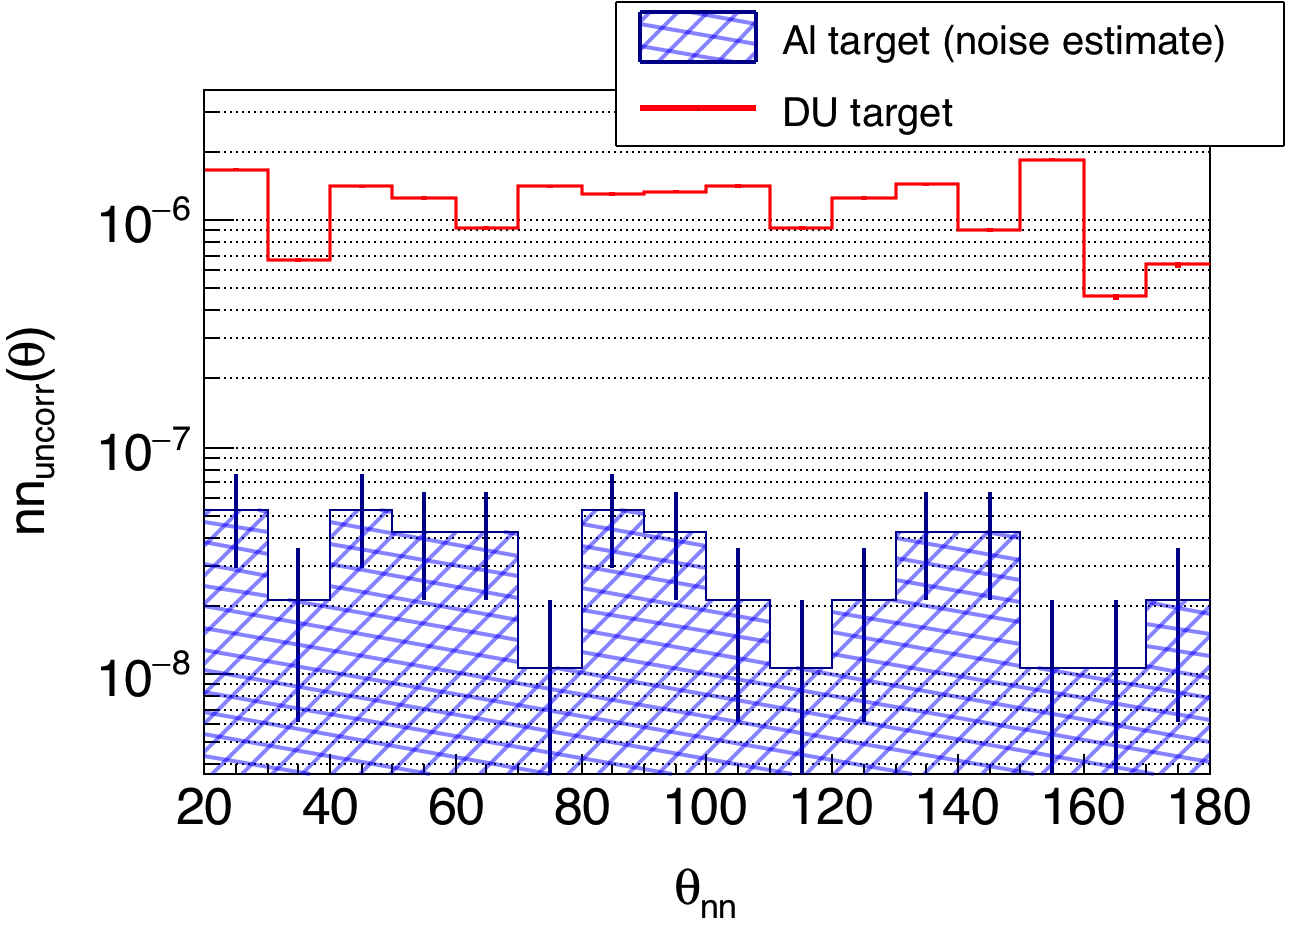
\includegraphics[width=0.8\textwidth]{Content/Methods/Noise.png}
    \caption{An Al target was designed to scatter the same number of photons as the DU target, thus serving as an equivalent non-neutron producing target sued to estimate noise.
    The rate of events with the Al target is 3\% that of the DU target. 
        }
    \label{fig:Noise}
\end{figure}

The efficiency and acceptance of the neutron detection system varies greatly over its opening angle range from 20$^{\circ}$ to 180$^{\circ}$, as illustrated in Fig.~\ref{fig:SPDPNormalization}(a).
This is due both to the neutron detection system's non-spherical symmetry, and to varying efficiency as a function of particle position on a detector.
In order to give a result that is sensitive to angular correlations but insensitive to detector efficiencies and experimental drifts, angular correlation is always expressed as a ratio between $nn_{\text{corr}}(\theta)$~and~$nn_{\text{uncorr}}(\theta)$.

Figure~\ref{fig:SPDPNormalization}(a) shows the measured $nn_{\text{corr}}(\theta)$ yield distribution of neutrons from the photofission of $^{238}$U.
The structure seen here is reflective of the underlying two-neutron angular correlations as well as the geometric acceptance and efficiencies of the neutron detectors.
Figure~\ref{fig:SPDPNormalization}(b) reveals how a clear picture of two-neutron correlations is produced by taking the ratio between $nn_{\text{corr}}(\theta)$ and $nn_{\text{uncorr}}(\theta)$.
\begin{figure}[]
\centering
    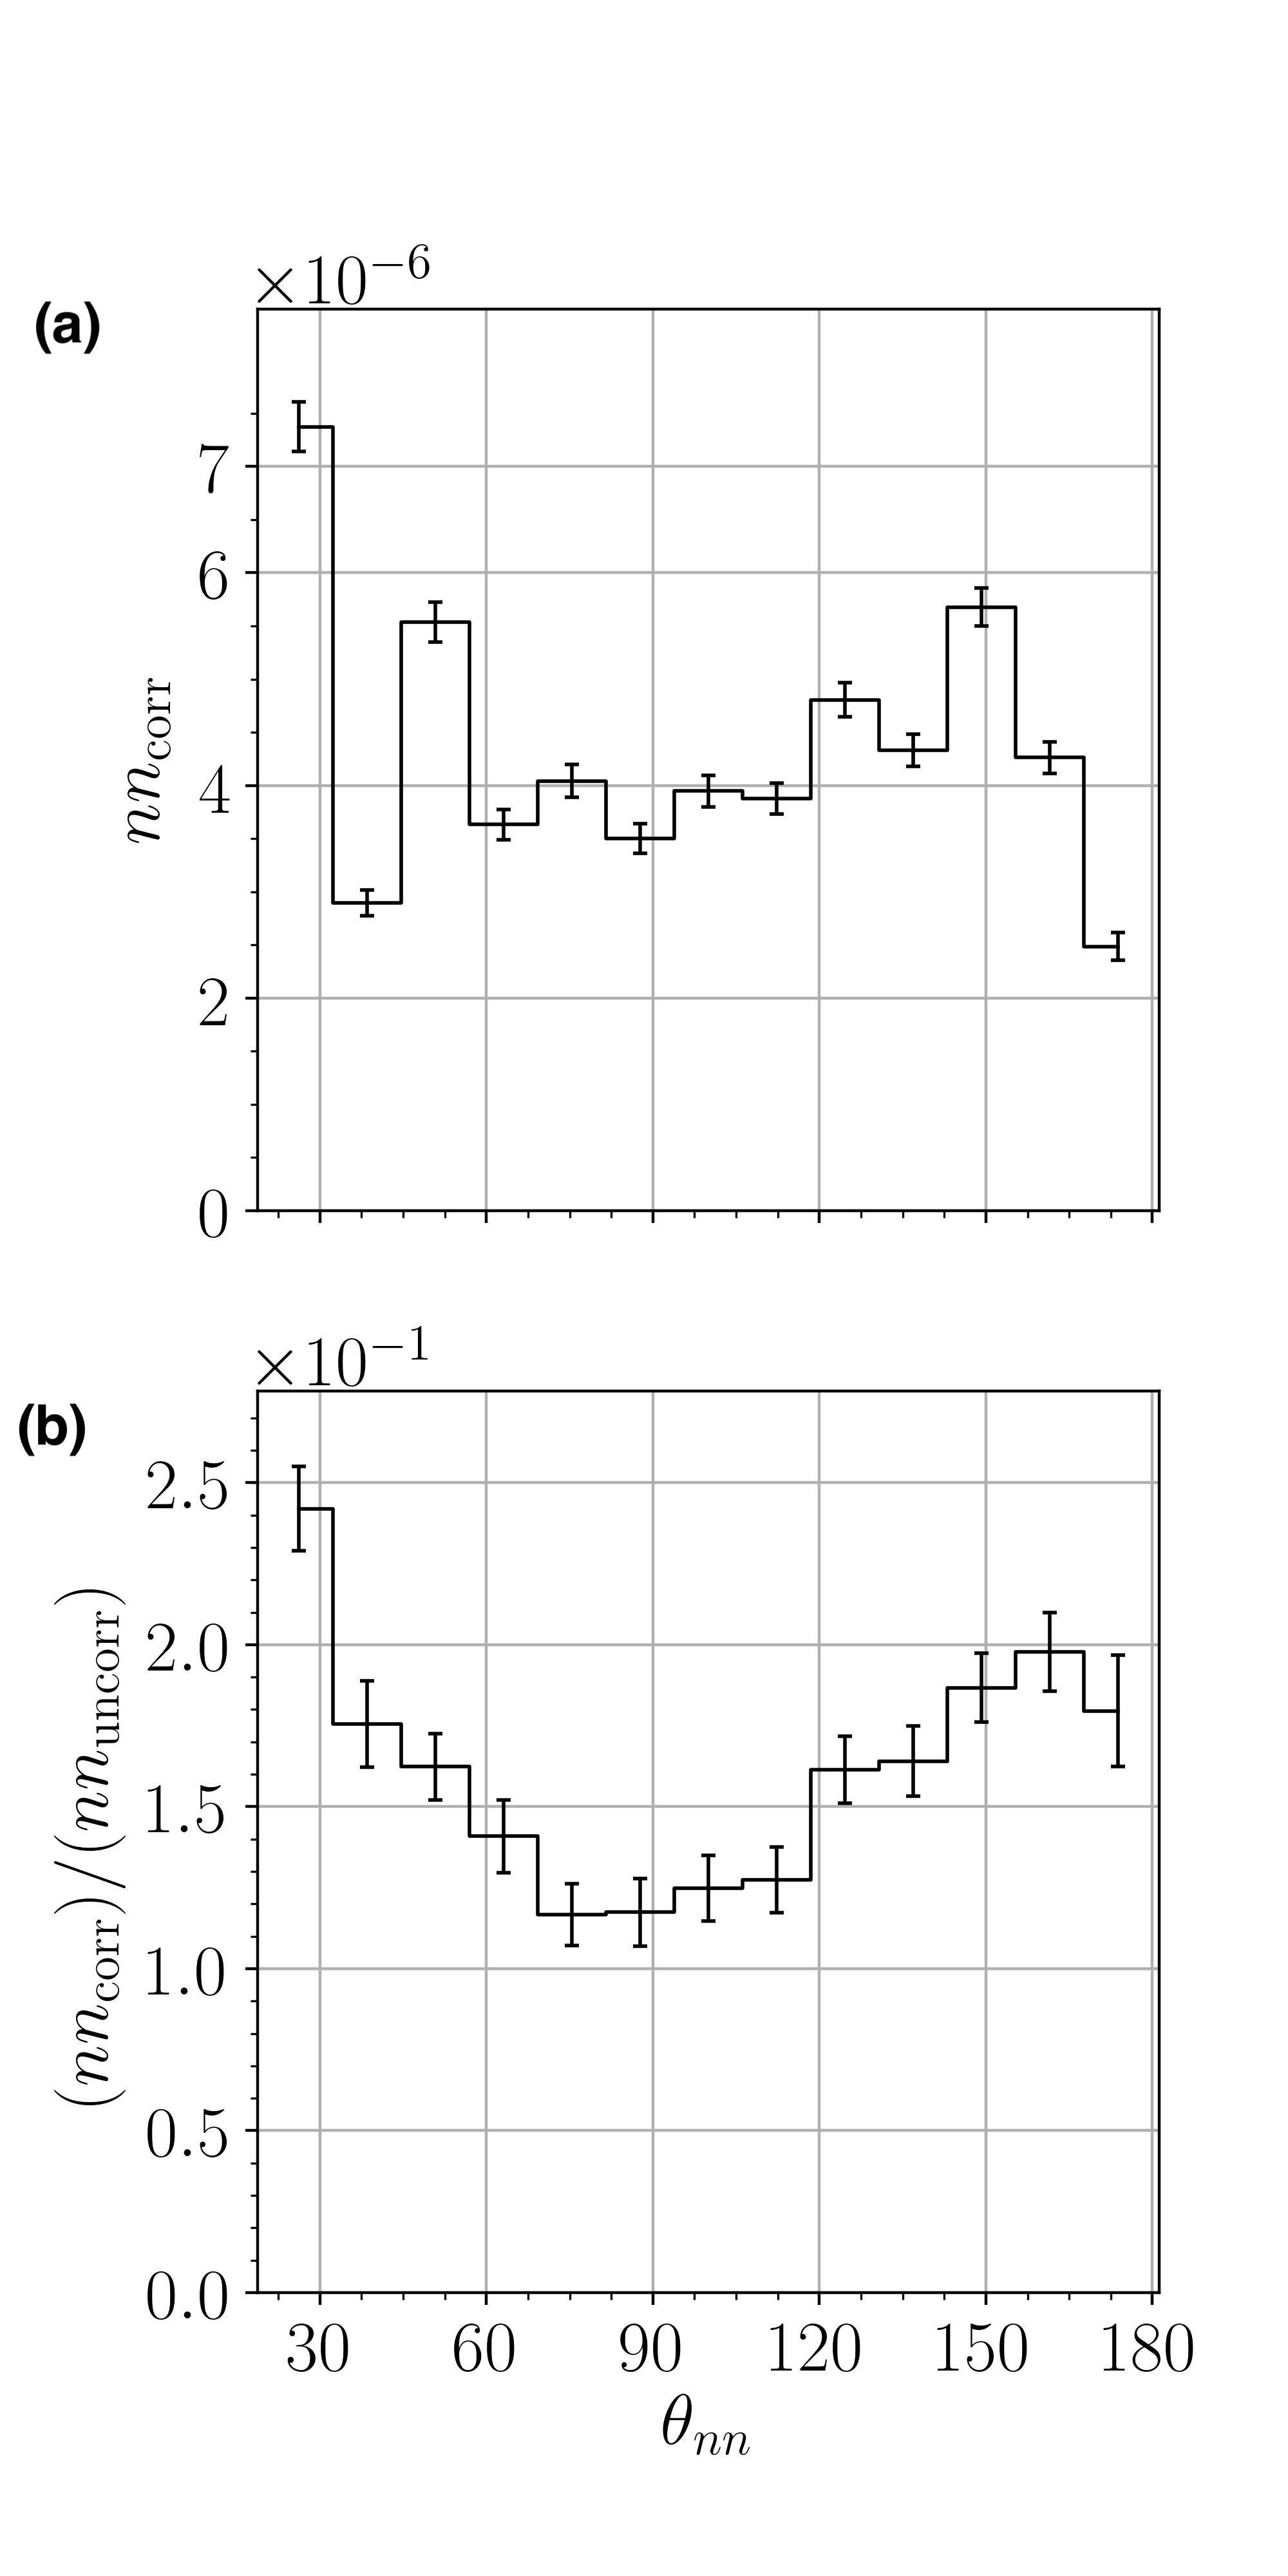
\includegraphics[width=0.965\textwidth]{Content/Methods/SPDPNormalization.png}
    \caption{(a) Two-neutron opening angle distribution from the photofission of $^{238}$U before normalization, and, (b) after normalization to the distribution of uncorrelated two-neutron events from different pulses. All neutrons have energy greater than 0.4 MeV.}
    \label{fig:SPDPNormalization}
\end{figure}

\subsection{Reconstruction of Accidental Coincidence Signal}
\label{Reconstruction of Accidental Coincidence}
The detection of two uncorrelated events in coincidence, whether the cause of which is neutrons, photons, or background signals, is referred to as an \emph{accidental}.
The reconstruction of the signal from accidentals as a function of opening angle, denoted by $nn_{\text{uncorr}}(\theta)$, is achieved using a manufactured set of opening angles, denoted by $nn_{\scaleto{DP}{4pt}}(\theta)$, which is produced by pairing events that occurred during different pulses.
This is done by examining pulses in pairs of two, which are required to have occurred within 0.2 seconds of each other, and for those pairs that have an event in both pulses, the opening angle is calculated between the events in the same way that it would be for coincident events from the same pulse.

The usefulness of $nn_{\scaleto{DP}{4pt}}(\theta)$ is that it is proportional to $nn_{\text{uncorr}}(\theta)$, and thus can be used to unfold the signal produced by correlated coincidences from a signal that is a mix of correlated and accidental coincidences.
Because accidental coincidences consist of two independent events, it does not matter whether the two events occurred during the same pulse or during two different pulses, given that the two different pulses occurred at around the same time and thus under the same experimental conditions.
Therefore, $nn_{\text{uncorr}}(\theta)$ will have an opening angle distribution with the same shape as  $nn_{\scaleto{DP}{4pt}}(\theta)$.
However, $nn_{\text{uncorr}}(\theta)$ is not equal to $nn_{\scaleto{DP}{4pt}}(\theta)$, because there are, on average, twice as many events in a pulse-pair than there are in a single pulse.
For this reason, as the following analysis shows,~$nn_{\text{uncorr}}(\theta) = \frac{1}{2}nn_{\scaleto{DP}{4pt}}(\theta)$.

The number of uncorrelated events detected per pulse is assumed to follow the Poissonian distribution, which describes the occurrence of independent random events.
Let $\lambda$ represent the mean number of uncorrelated events per pulse. 
To determine the value of $\lambda$, one needs to know whether a given coincident event is in fact an accidental, as $\lambda$ only quantifies the rate of accidental coincidences.
Such information is not known, but the largest possible value for $\lambda$ is the mean number of events per pulse, as this assumes all events are uncorrelated.
This placed an upper bound on $\lambda$ of $3\times 10^{-6}$, which is small enough to neglect all terms on the order of $\lambda^3$ or greater.

The per-pulse accidental coincidence rate from individual pulses summed over all opening angle bins, denoted by $\sum_{\theta} nn_{\text{uncorr}}(\theta)$, is equal to the poissonian probability of there being exactly two uncorrelated events detected in a single pulse\footnote{For the sake of brevity, cases of greater than two-fold coincidence are not considered in this analysis, and it is not necessary to do so because of the low detection rates during this work. It can be shown, however, that accounting for any number of coincidences, from zero all the way up to $\infty$-fold coincident events in a pulse or pulse-pair, gives the same answer.}:
\begin{equation} \label{math:SP}
    \begin{split}
    \sum_{\theta} nn_{\text{uncorr}}(\theta) & = \frac{e^{-\lambda}\lambda^{2}}{2!} \\
        &\approx \frac{\lambda^2}{{2}} + \mathcal{O}(\lambda^3) \, .
    \end{split}
\end{equation}
For the case of different-pulse pairs, a ``coincidence'' occurs when there is an event in both pulses. Cases in which there are more than two events can be neglected due to their rare occurrence in this work, therefore, the total per-pulse rate for different-pulse pairs is the square of the poissonian probability of there being one event:
\begin{equation} \label{math:DP}
    \begin{split}
   \sum_{\theta} nn_{\scaleto{DP}{4pt}}(\theta)&= \left(e^{-\lambda}\lambda\right)^{2} \\
    &\approx \lambda^2 + \mathcal{O}(\lambda^3) \, .
    \end{split}
\end{equation}
For the reasons explained above, $nn_{\scaleto{DP}{4pt}}(\theta)$ and $nn_{\text{uncorr}}(\theta)$ have the same shape, thus, from Eq.'s (\ref{math:DP}) and (\ref{math:SP}) it follows that 
\begin{equation}
\label{eq:uncorr_DP}
nn_{\text{uncorr}}(\theta) = \frac{1}{2}nn_{\scaleto{DP}{4pt}}(\theta) \,.
\end{equation}
%Before the different-pulse distribution can be subtracted from the same-pulse distribution, removing the effects of accidental coincidences on the result, both distributions must be properly normalized.
%The $\theta_{nn}$ distribution of coincident events from the same pulse is normalized to the number of pulses.
%The $\theta_{nn}$ distribution from different-pulse events is normalized to the amount of pulse-pairs examined, and is then multiplied by a weighting factor, $w$, equal to 1/2.
%After the subtraction of accidental coincidences, the final step in the analysis is to divide the result by the different-pulse distribution to remove the effects of detector efficiencies and experimental drifts 

\subsection{Accidental Coincidence Subtraction}
\label{accidental subtraction}
The accelerator's current was adjusted so that there are, on average, less than 1.0 fissions per pulse.
Nevertheless, statistical fluctuations in the number of fissions per pulse result in some contamination of the data by accidental coincident neutrons that originated from different, and therefore, uncorrelated fissions.
There are also uncorrelated neutrons produced when multiple $(\gamma, n)$ reactions occur in a single pulse.
The $^{238}$U cross-section of $(\gamma, n)$, integrated over the relevant bremsstrahlung energy distribution, is about a factor of 7 times greater than it is for photofission.
As a result, it was unavoidable that there be a significant number of neutron coincidences caused by multiple $(\gamma, n)$ reactions relative to those caused by correlated fission neutrons.

If not subtracted from the result, the opening angle distribution of uncorrelated neutrons will wash out the signal from correlated neutrons. 
As described earlier in section~\ref{Reconstruction of Accidental Coincidence}, the signal due to uncorrelated neutron coincidences, $nn_{\text{uncorr}}(\theta)$, can be reconstructed by looking at pulses in pairs, $nn_{\scaleto{DP}{4pt}}(\theta)$.
Using Eq.'s~(\ref{eq:corr_uncorr})~and~(\ref{eq:uncorr_DP}),  $nn_{\text{corr}}(\theta)$ can be expressed in terms of measured quantities:
\begin{equation} \label{math:SP}
    \begin{split}
    nn_{\text{corr}}(\theta) &=  nn_{\text{raw}}(\theta) - nn_{\text{uncorr}}(\theta) \\
    &= nn_{\text{raw}}(\theta) - \frac{1}{2}nn_{\scaleto{DP}{4pt}}(\theta) \, .
    \end{split}
\end{equation}

\subsection{Correction for Uncorrelated Neutron Energy Distribution}
The measured yield of correlated neutron pairs as a function of the energy of both neutrons,  denoted by $Y_{\text{2n-corr}}(E_1,E_2))$, is different from that of uncorrelated neutron pairs, denoted by $Y_{\text{2n-uncorr}}(E_1,E_2))$.
There are two reasons for this.
The first is that, because $Y_{\text{2n-uncorr}}(E_1,E_2))$ consists of uncorrelated neutron pairs, it has the form
\begin{equation}
	 Y_{\text{2n-uncorr}}(E_1,E_2) = Y_{\text{n-uncorr}}(E_1) Y_{\text{n-uncorr}}(E_2) \, .
\end{equation}
The second reason is that, unlike $Y_{\text{2n-corr}}(E_1,E_2))$, $Y_{\text{2n-uncorr}}(E_1,E_2) $, is influenced by the presence of accidental neutron coincidences due to multiple $(\gamma, 1)$ reactions in a single pulse, which produce neutrons of a lower mean energy than fission neutrons.
The two-neutron detection efficiency depends on the energy of both neutrons, so it would not necessarily be true that the effects of detector efficiency cancel in the fraction $\frac{nn_{\text{corr}}(\theta)}{nn_{\text{uncorr}}(\theta)}$ as previously stated.
The solution is to apply a weight to each uncorrelated two-neutron event, such that $Y_{\text{2n-uncorr}}(E_1,E_2))=Y'_{\text{2n-corr}}(E_1,E_2))$,
where $Y'_{\text{2n-corr}}(E_1,E_2))$ is the weighted yield of uncorrelated neutrons as a function of the energy of both neutrons.
This correction produces a small effect that is only significant for neutrons at small angles above about 3.6~MeV. 

